\section{Data and Methodology}
%THIS SHOULD DESCRIBE THE SATELLITE DATA AND THE TECHNIQUES USED TO PROCESS AND ANALYSE THESES DATA.
\subsection{Observations and Data Reduction}
Using data collected by spacecraft observing the Sun, energy released during solar flares can be tracked as it is deposited throughout the atmosphere. The X1 flare of the 29th of March 2014 in active region NOAA 12017, was well observed by RHESSI, IRIS and SDO/HMI, collecting HXR, UV and optical emission respectively. The peak of the impulsive phase of the flare occurs at 17:48 UT, at which point all mentioned instruments provide good coverage. 

\subsubsection{The Ramaty High Energy Solar Spectroscopic Imager}
%insert RHESSI background info
The Ramaty High Energy Solar Spectroscopic Imager (RHESSI) observes solar emission ranging from 1 keV X-rays to 20MeV $\gamma$-rays produced by energetic particles and nuclear interactions. RHESSI was designed with the aim of understanding impulsive energy release, particle acceleration and transportation in the magnetohydrodynamic environment of the solar atmosphere. Isolating the 10 - 100 keV energy data collected by RHESSI can provide information regarding the intensity and spatial origin of a HXR source. This allows the location of magnetic HXR footpoints to be tracked and the calculation of energy depostion by accelerated electrons. During the impulsive phase of a flare, high energy x-ray emission is an indicator that accelerated particles are present. Assuming that the chromosphere is a thick target \citep{1971SoPh...18..489B}, the deposition of energy by accelerated particles is due to collisions between charged particles and ions producing hard X-ray bremsstrahlung emission. Using equation \ref{pnth} one can calculate the power, $P$, injected into the atmosphere by non-thermal electrons.  
 
\begin{equation}\label{pnth}
P(E \geq E_{c}) = \int_{E_{C}}^{\infty} EF(E)dE
\end{equation}

The electron distribution $F(E)$ is controlled by the power law $AE^{-\delta}$, where $E$ is the electron energy, $A$ is the total injected electron rate normalisation factor, $E_{C}$ is the low energy cut off and $\delta$ is the electron distribution spectral index. The value of $E_{C}$ represents the upper boundary between thermal and non-thermal energy contributions to the x-ray spectrum. This means that the total energy associated with non-thermal electron power is a lower limit. Performing the integral in equation \ref{pnth} gives the total non-thermal electron power in the form of equation \ref{pnth1}.

\begin{equation}\label{pnth1}
P(E \geq E_{c}) = \frac{AE_{C}^{(2-\delta)}}{(\delta - 2)}
\end{equation}

Once $P$ has been determined, a total energy can be calculated by multiplying the power by the time period over which the data covers. In this case that would be the impulsive phase of the flare.
  
Practically applying a thick target model fit to RHESSI data is acheived by using the \texttt{ospex} software within SolarSoft (SSWIDL). The entire data set has to be split into short intervals to improve the accuracy of fitting and the detail of resulting plots. The attenuator state of the instrument has to be taken into account due to differences in sensitivity to incoming photons. Therefore it is important to define intervals for fitting first by the attenuator state as \texttt{ospex} will mitigate for the differences in count sensitivity. Then each attenuator time period can be split further in to smaller time increments. Shown in Figure \ref{erhessi} is the resulting fit over the impulsive phase of the flare. At the peak of the impulsive phase between 17:46 and 17:48 the RHESSI fit shows an energy ranging from $1.0{\times}10^{28}$ to $2.5{\times}10^{29}$ erg. Assuming the fitting model is correct then the release of this energy is due to non-thermal electrons being accelerated by magnetic reconnection, depositing their energy into the chromosphere. 

\begin{figure}[H]
  \begin{center}
  \textbf{RHESSI 10 - 100 keV Hard Xray Energy Over Time}\par\medskip
  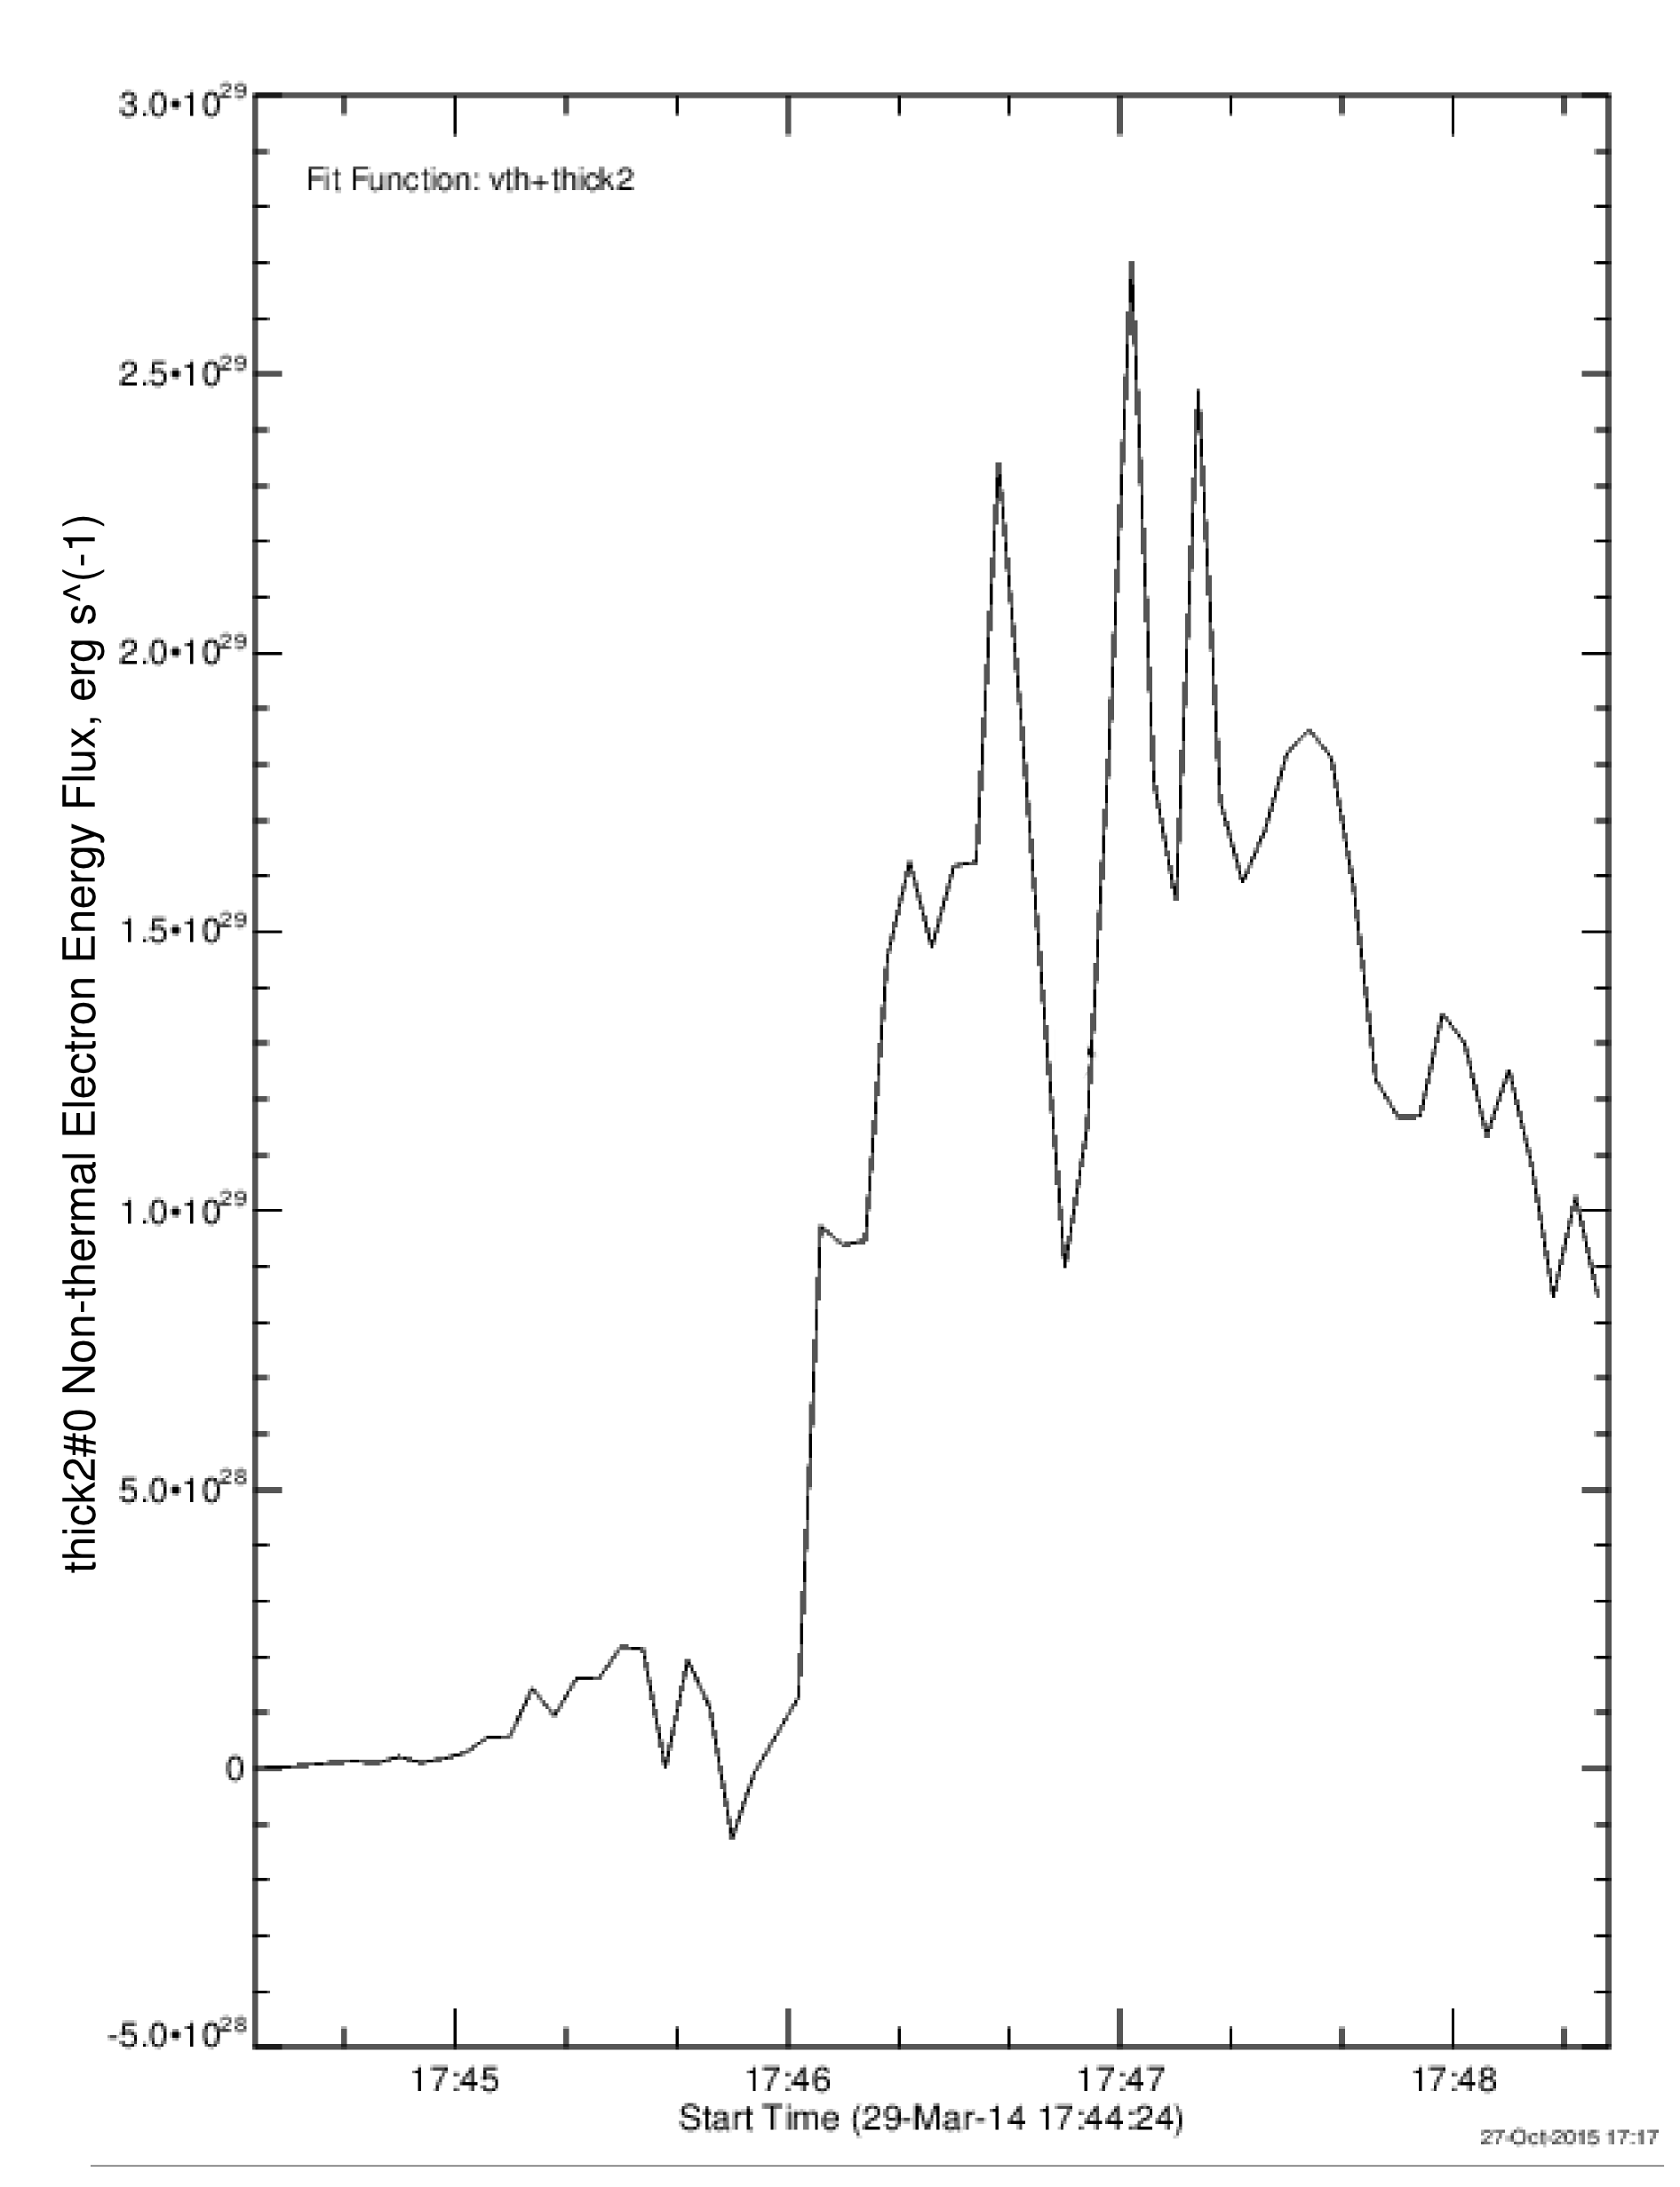
\includegraphics[width=0.6\textwidth]{rhessi-energy-curve}
  \end{center}
  \caption{Shows the energy evolution of hard x-ray emission collected by RHESSI 10 to 100 keV bins. Energy units are calculated by fitting a non-thermal electron model to the data. }\label{erhessi}
\end{figure}


\subsubsection{The Interface Region Imaging Spectrograph}
Observing UV ribbons requires a different spacecraft. The Interface Region Spectroscopic Imager (IRIS) captures near-ultraviolet (NUV) and far-ultraviolet (FUV) emission and is designed to observe the chromosphere at various altitudes. Emission is collected by a slit-jaw imager (SJI) and a spectrometer (SG) simultaneously. The spectrograph is sensitive in both FUV and NUV passbands, which expose 3 CCDs to produce spectra in three UV bands, two FUV and one NUV. Table \ref{iris-sg} shows how each passband relates to emission processes occurring from the upper-chromosphere down to the upper-photosphere.

\begin{table}[H]
\centering
\begin{tabular}{|c|c|c|c|}
Band & Wavelength \AA\ & Temperature $\log{T}$ & Region of Atmosphere\\
\hline
FUV 1 & $1331.7 - 1358.4$ & $3.7 - 7.0$ & Upper to lower-chromosphere\\
FUV 2 & $1389.0 - 1407.0$ & $3.7 - 5.2$ & Upper to lower-chromosphere\\
NUV & $2782.7 - 2851.1$ & $3.7 - 4.2$ & Chromosphere to upper-photosphere\\
\end{tabular}
\caption{The IRIS/SG is capable of observing three passbands, which relate to different plasma temperatures.}\label{iris-sg}
\end{table}


The slit-jaw images, are light collected from a reflective area surrounding the slit. The imager is capable of observing four wavelengths relating to emission at different altitudes as shown by Table \ref{iris-sj}.

\begin{table}[H]
\centering
\begin{tabular}{|c|c|c|c|c|}
SJI Passband & Wavelength \AA\ & FWHM \AA\ & Temperature $\log{T}$ & Region of Atmosphere\\
\hline
C II  & $1330$ & $40$ & $3.7 - 7.0$ & Upper-chromosphere\\
Si IV  & $1400$ & $40$ & $3.7 - 5.2$ & Upper-chromosphere\\
Mg II h/k & $2796$ & $4$ & $3.7 - 4.2$ & Lower-chromosphere\\
Mg II wing & $2832$ & $4$ & $3.7 - 3.8$ & Upper-photosphere\\
\end{tabular}
\caption{The IRIS/SJ is capable of observing four passbands, which relate to different plasma temperatures.}\label{iris-sj}
\end{table}


The IRIS spacecraft captured the temporal evolution of the flare between 14:09 and 17:54 UT via it's slit-jaw imager and spectrograph at solar coordinates 491", 282", with a spatial resolution of 0.1667" per pixel. The slit-jaw imager data provides coverage of a field of view spanning 167" by 174", of passbands that including 1403, 2796 and 2832 \AA\ at 26, 19 and 75 second cadence respectively. The spectrograph slit has a field of view spanning 14" by 174" and is aligned directly over chromospheric flare ribbons, and the sunquake point of origin. For the majority of the observation, the spectrograph slit is exposed for $\sim9$ seconds at 8 slit locations for a total of 72 seconds cadence per raster. However, during the impulsive phase the IRIS SG shortens it's exposure time to around 2.4 seconds in order to mitigate against saturation of the CCDs. Wavelengths observed over three channels include FUV1: 1331.7 - 1358.4 \AA, FUV2: 1389.0 - 1407.0 \AA\ and NUV: 2782.7 - 2851.1 \AA, associated with the transition region, chromosphere and the upper-photosphere. Spectral lines include C II, Si IV and Mg II h and k. IRIS SJI data is the standard level 2 data product provided for scientific research, which has been calibrated to negate dark currents, flat-field and spacecraft rotational effects. In order to observe flare ribbons in the photospheric data captured by IRIS SJI MG II wing channel, a running difference filter is applyed. This effectively removes unwanted background features, highlighting the UV ribbons. IRIS SG data is manually corrected for changing exposure times and wavelength shifts caused by the orbital motions of the spacecraft. IRIS SG data is sampled over a wavelength range of 2825.7 and 2825.8\AA\ which represents a sample of Balmer pseudo-continuum. The next stage of the processing requires that IRIS SJ and SG data are converted from relative intensity (DN per pixel) to energy (erg) units. This is acheived by using a method provided in the instrument documentation \citep{2014SoPh..289.2733D} which calculates the conversion factors between DN and erg units in SSWIDL. It is then a case of inserting IRIS DN per pixel intensity values into the equation \ref{irisradiometriccal} converting them into energy units. $F_{DN}$ is flux in units of DN per pixel, $C_{d2p}$ is the DN to photon conversion factor, $E_{\lambda}$ is the photon energy and $E_{erg}$ is to put the result into erg units.  

\begin{equation}\label{irisradiometriccal}
E = \frac{F_{DN}  C_{d2p} E_{\lambda}}{E_{erg}}
\end{equation}


\subsubsection{The Solar Dynamics Observatorie's Helioseimic and Magnetic Imager}
Signatures of energy deposition in the lowest regions of atmosphere are captured by Solar Dynamics Observatory's (SDO) Helioseismic Imager (HMI), which is sensitive to the wing of the photospheric absorption line 6173 \AA\ (Fe I), which is essentially optical continuum. SDO/HMI has three main observables, continuum, dopplergrams and magnetic field configuration, each of which can provide valuable insight into the physical conditions existing in photospheric plasma. In particular for this project, optical continuum data can provide information about WLFs intensity, which along with Balmer continuum could be linked to radiative backwarming of photospheric material, which is a possible sunquake progenitor. The point of origin and wave-fronts of the sunquake can also be detected using helioseismic data, which can be used to calculate acoustic power of the quake.
The HMI instrument onboard SDO observes the entire solar photosphere with 4k resolution and a pixel size relating to 0.505" by 0.505", with each image having a cadence of 45 seconds. The data is calibrated to negate cosmic-rays, dark currents, flat-field and spacecraft rotational effects. In this project, HMI continuum data is used primarily to observe White light flares, which are difficult to see against the bright photospheric background. To highlight the positions of flare ribbons in the photosphere, data must be filtered. Silimarly to \cite{2014ApJ...783...98K}, photospheric continuum data captured by HMI is put through a two stage filtering porcedure. First the data has an unsharp filter applied, so that the filtered image, $I_{filt}=I-$ smooth($I$,10), where $I$ is the original image and the function smooth relates to a 10 pixel boxcar smoothing filter, this is to remove small features such as granulation. The technique is not perfect meaning that some granulation is still visible after the unsharp filter. Second, $I_{filt}$ is subjected to a running difference filter to isolate locations that are white-light enhanced. The running difference filter effectively removes static features leaving behind those pixels that are changing over short time-scales. However, for removing signatures of those processes occurring over shorter time periods such as the remaining granulation and also p-mode oscillations, this filtering technique is ineffective. This is not a problem, as for the purpose of white light flare analysis, the data yield a strong contrast between flare-enhanced and background pixels after being filtered by a $i-2$ running difference. The next stage is to determine which pixels in the difference image are those that are enhanced during the flare. For the best result, white-light enhanced pixels are identified using a combination of visual inspection and thresholding. Attempts at automating the identification process tend to lead to false positives being triggered by noise or granulation features. \\
HMI Dopplergrams are used in conjunction with holography techniques to produce a 6mHZ acoustic egression power map (supplied via private communication by Sergei Zharkov) revealing the location of the sunquake. 
As with the IRIS data, the next stage of processing is to calculate and energy. To perform the energy conversion for SDO HMI data a combination of sources \citep{2012SoPh..275...41B, 2012SoPh..275..285C} have been used to find the instrument's properties which are used to fulfil a conversion factor in the form of equation \ref{hmiradiometriccal}. Where $g$ is the instrument gain, $QE$ is the quantum efficiency of the charged couple device and $A_{ap}$ is the instrument aperture area, all other terms hold the same meaning as in equation \ref{irisradiometriccal}.

\begin{equation}\label{hmiradiometriccal}
E = \frac{F_{DN} E_{\lambda}}{g QE A_{ap} E_{erg}}
\end{equation}

\subsection{Data Sampling}
For the IRIS SJI, IRIS SG and SDO HMI data sets, multiple sample points have been chosen based on the moment in time when the IRIS SG slit is directly over the southern flare ribbon and sunquake impact location. These coordinates are sampled across all data sets except RHESSI due to the limited spatial resolution of the instrument. Figure \ref{mgrib} shows the sample coordinates, RHESSI HXR and the 6mHz sunquake egression map, plotted over IRIS SJI MG II data in an effort to demonstrate the spatial alignment between HXR (particle beam), UV ribbons and sunquake impact. Table \ref{coordtab} shows how each sample number relates to a heliocentric position in arcseconds.
\centering

\begin{table}
\begin{tabular}{|c|c|}
\hline
Sample Number & Heliocentric Position (x,y)\\
\hline
1 & 518.219", 262.000"\\
2 & 520.215", 263.000"\\
3 & 522.212", 262.000"\\
4 & 522.212", 265.000"\\
5 & 524.256", 265.000"\\
6 & 526.252", 263.818"\\
\hline
\end{tabular}
\caption{Sample number and the corresponding coordinates in heliocentric units (arcsec).}\label{coordtab}
\end{table}

\begin{figure}[H]
  \begin{center}
  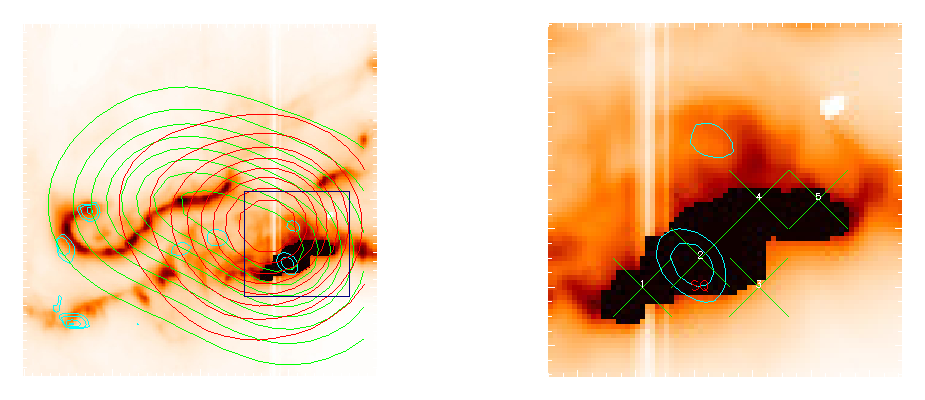
\includegraphics[width=0.8\textwidth]{29-Mar-14-MGII-Sunquake-Context-Plots-xx-Zoom-crop}
  \end{center}
  \caption{The images show IRIS Mg II slit-jaw data with contours representing HXR emission and 6mHz sunquake power. The black box highlights the area contained in the zoomed plot on the right. The cyan contours show the 6mHz egression power, with the location of the sunquake shown in red on the right. The green and red contours on the left plot show RHESSI HXR data at 25 - 50 and 50 - 100 keV. The green crosses on the right plot show sample positions numbered in accordance with table \ref{coordtab} Each of the IRIS SJ and SDO HMI data sets are sampled at the exact same coordinates in heliocentric units.}\label{mgrib}
\end{figure}


\subsection{Results and Discussion}
\subsection{Interpretation and Discussion}
\subsection{Conclusions and Thesis Plan}



